\chapter{Анализ трёх аспектов современных стран по Викиданным: возраст стран, популярные формы правления и этнохоронимы}
\label{ch:country}

Эта глава посвящена исследованию стран на основе базы знаний международного проекта Викиданные. С помощью SPARQL-запросов, вычисляемых на объектах типа ”страна” в Викиданных, получены: выведен список всех ныне существующих стран, перечень стран, упорядоченных по дате создания, список этнохоронимов стран, пузырьковая диаграмма с формами правления стран и граф соседних стран. Кроме того, сделаны отностительно полноты Викиданных по данной теме.

\section{Формы правления стран}

Построим пузырьковую диаграмму форм правления стран.

Используются:
\begin{itemize}
	\item объект country (Q6256) (страна);
	\item свойство subject's government (P122) (форма правления).
\end{itemize}

В итоге получим SPARQL-запрос, 30 записей (2017), 29 записей (2020)

В результате выполнения запроса мы получаем пузырьковую диаграмму с наиболее распространенными формами правления в странах по 2017 году на рис. ~\ref{fig:bubble_chart_forms_of_government_countries_2017}, по 2020 году на рис.~\ref{fig:bubble_chart_forms_of_government_countries_2020}.

\begin{figure}
	{
		\setlength{\fboxsep}{0pt}%
		\setlength{\fboxrule}{1pt}%
		\fcolorbox{gray}{gray}{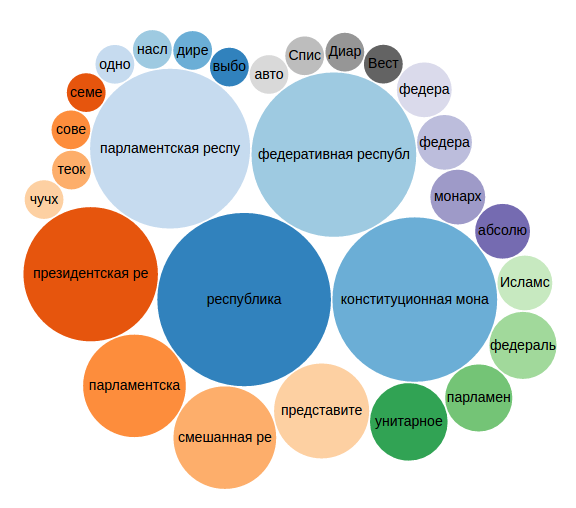
\includegraphics[width=\linewidth]{./chapter/country/Bubble_chart_forms_of_government_countries_according_to_Wikidata.png}}%
	}
	\caption{Пузырьковая диаграмма форм правления стран, 2017.
		\\			
		По данным на 2017 год основные формы правления стран: республика (в 20 странах), конституционная монархия (в 18 странах), федеративная республика (в 18 странах), парламентская республика (в 17 странах) и президентская республика (в 12 странах).}%
	\label{fig:bubble_chart_forms_of_government_countries_2017}%
\end{figure}

\begin{figure}
	{
		\setlength{\fboxsep}{0pt}%
		\setlength{\fboxrule}{1pt}%
		\fcolorbox{gray}{gray}{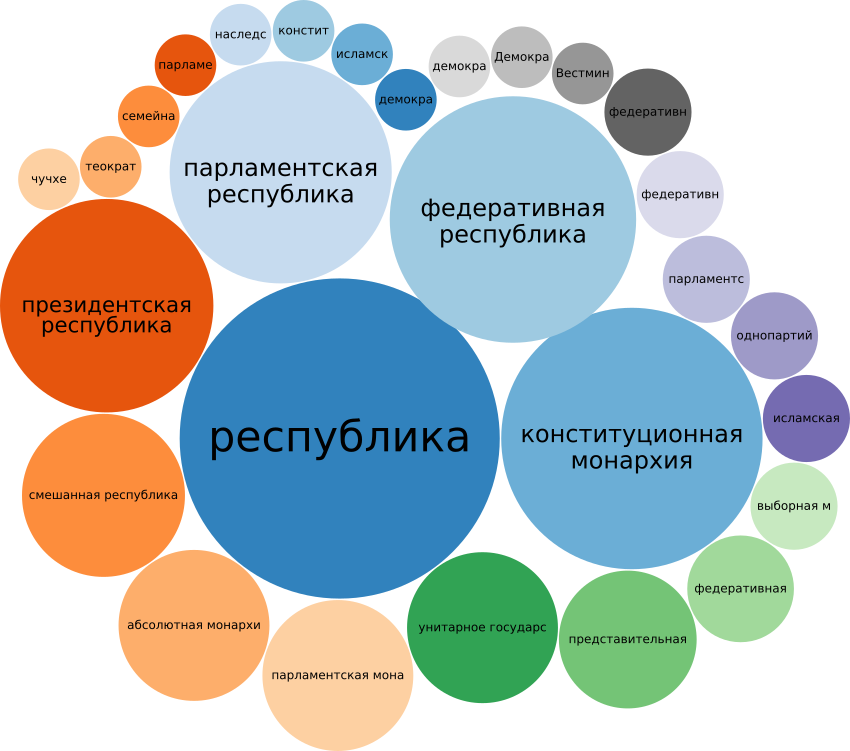
\includegraphics[width=\linewidth]{./chapter/country/Bubble_chart_forms_of_government_countries_according_to_Wikidata_2020.png}}%
	}
	\caption{Пузырьковая диаграмма форм правления стран, 2020.
	\\
	По данным на 2020 год  основные формы правления стран: республика (в 27 странах), конституционная монархия (в 18 странах), федеративная республика (в 16 странах), парламентская республика (в 13 странах) и президентская республика (в 12 странах).
}%
	\label{fig:bubble_chart_forms_of_government_countries_2020}%
\end{figure}